%% FullCourse_10Lecs -- Lecture 8, Act 8.4 (GENERATE): Grounded Answers and RAG vs Fine-Tuning.
%% Rebuilt 2026-07-08 per Lec08_Rewrite_Plan_2026-07-08.md ("one map, five acts").
%% Source: archive_pre_split/pre_map_rebuild_2026-07-08/Lec08_T4a_Augmented_Gen_Apps.tex
%% (frames f2-f10 + f19; the six economic use cases, three-roles taxonomy, and
%% workflow-patterns synthesis moved to the new T5).

%% Shared preamble for the FullCourse_10Lecs topic decks.
%%
%% Each topic .tex \input's this file, then defines its own \title, \date
%% override (if any), \graphicspath, and \begin{document}.
%%
%% Reconstructed verbatim from the inlined copy preserved in
%% Lec10_Case_Studies/Lec10_T8_Case6_DeepRamsey.tex (lines 23-190), which is
%% explicitly annotated there as "from ../shared_preamble.tex, copied verbatim".
%% Base preamble matches MiniCourse_8hr/Slides/shared_preamble.tex; this version
%% additionally provides \sectiondivider, the conceptbox/cautionbox/examplebox/
%% takeawaybox tcolorboxes, and \compacttables used across the split decks.

\documentclass[10pt,english,aspectratio=169]{beamer}

\usepackage{ae,aecompl}
\usepackage[T1]{fontenc}
\usepackage{textcomp}
\usepackage[utf8]{inputenc}
\usepackage{babel}
\usepackage{datetime2}

\setcounter{secnumdepth}{3}
\setcounter{tocdepth}{3}

\usepackage{amsmath, amssymb, amsthm, graphicx}
\usepackage{booktabs, multirow}
\usepackage{tikz}
\usepackage{pgfplots}
\pgfplotsset{compat=1.16}
\usepackage[most]{tcolorbox}
\tcbuselibrary{skins, breakable, theorems}
\usepackage{listings}
\usepackage{xcolor}

\lstset{
  basicstyle=\ttfamily\small,
  keywordstyle=\color{blue!80!black}\bfseries,
  commentstyle=\color{green!50!black}\itshape,
  stringstyle=\color{orange!80!black},
  backgroundcolor=\color{gray!8},
  frame=single,
  rulecolor=\color{gray!40},
  breaklines=true,
  showstringspaces=false,
  numbers=none,
}

\lstdefinestyle{pythonstyle}{
    language=Python,
    basicstyle=\ttfamily\footnotesize,
    keywordstyle=\color{blue!80!black}\bfseries,
    commentstyle=\color{green!50!black}\itshape,
    stringstyle=\color{orange!80!black},
    frame=single,
    breaklines=true,
    showstringspaces=false,
    numbers=left,
    numbersep=5pt,
    numberstyle=\tiny\color{gray},
    backgroundcolor=\color{gray!8},
    rulecolor=\color{gray!40}
}

\ifx\hypersetup\undefined
  \AtBeginDocument{%
    \hypersetup{bookmarks=false,breaklinks=true,pdfborder={0 0 0},colorlinks=true,
      linkcolor=DarkText,urlcolor=RedTitle}%
  }
\else
  \hypersetup{bookmarks=false,breaklinks=true,pdfborder={0 0 0},colorlinks=true,
    linkcolor=DarkText,urlcolor=RedTitle}%
\fi

\makeatletter
\newcommand\makebeamertitle{%
  \begin{frame}[plain]
    \vspace*{1.0cm}
    \centering
    {\usebeamerfont{title}\usebeamercolor[fg]{title}\inserttitle\par}
    \vspace{1.0cm}
    {\usebeamerfont{author}\usebeamercolor[fg]{author}\insertauthor\par}
    \vspace{0.2cm}
    {\usebeamerfont{date}\usebeamercolor[fg]{date}\insertdate\par}
  \end{frame}}%
\AtBeginDocument{%
  \let\origtableofcontents=\tableofcontents
  \def\tableofcontents{\@ifnextchar[{\origtableofcontents}{\gobbletableofcontents}}
  \def\gobbletableofcontents#1{\origtableofcontents}%
}

\usetheme{metropolis}
\usefonttheme{professionalfonts}

\definecolor{LightGray}{RGB}{230,230,230}
\definecolor{RedTitle}{RGB}{0,0,200}
\definecolor{VeryLightGray}{RGB}{245,245,245}
\definecolor{DarkText}{RGB}{0,0,0}

\setbeamercolor{background canvas}{bg=white}
\setbeamercolor{title}{fg=RedTitle}
\setbeamercolor{author}{fg=DarkText}
\setbeamercolor{date}{fg=DarkText}
\setbeamercolor{frametitle}{bg=VeryLightGray,fg=DarkText}
\setbeamercolor{normal text}{fg=DarkText}
\setbeamerfont{title}{size=\large}

\setbeamersize{text margin left=5mm, text margin right=5mm}
\addtobeamertemplate{frametitle}{}{\vspace{-0.5em}}
\newcommand{\reducevspace}{\vspace{-0.5cm}}

% Shared section divider and box styles for split topic decks.
\newcommand{\sectiondivider}[2]{%
\begin{frame}[plain,noframenumbering]
\begin{center}
\vfill
{\Large\textbf{#1}\par}
\vspace{0.35cm}
{\normalsize #2\par}
\vfill
\end{center}
\end{frame}
}

\newtcolorbox{conceptbox}[1][]{
  colback=blue!3,
  colframe=RedTitle!55,
  boxrule=0.35mm,
  arc=1mm,
  left=2mm,
  right=2mm,
  top=1mm,
  bottom=1mm,
  #1
}
\newtcolorbox{cautionbox}[1][]{
  colback=red!3,
  colframe=red!50!black,
  boxrule=0.35mm,
  arc=1mm,
  left=2mm,
  right=2mm,
  top=1mm,
  bottom=1mm,
  #1
}
\newtcolorbox{examplebox}[1][]{
  colback=green!3,
  colframe=green!45!black,
  boxrule=0.35mm,
  arc=1mm,
  left=2mm,
  right=2mm,
  top=1mm,
  bottom=1mm,
  #1
}
\newtcolorbox{takeawaybox}[1][]{
  colback=VeryLightGray,
  colframe=RedTitle!55,
  boxrule=0.35mm,
  arc=1mm,
  left=2mm,
  right=2mm,
  top=1mm,
  bottom=1mm,
  #1
}
\newcommand{\compacttables}{\renewcommand{\arraystretch}{1.15}}

\setbeamertemplate{navigation symbols}{}
\setbeamertemplate{footline}{%
  \hfill%
  \usebeamercolor[fg]{page number in head/foot}%
  \usebeamerfont{page number in head/foot}%
  \insertframenumber\,/\,\inserttotalframenumber\kern1em\vskip2pt%
}

\makeatother

\author{Zhigang Feng}
% "date with time": compile timestamp so each build is identifiable.
\date{\today\ \DTMcurrenttime}

\metroset{sectionpage=none}

% colortbl for \cellcolor in the RAG vs FT decision matrix
\usepackage{colortbl}

\usetikzlibrary{arrows.meta, positioning, shapes, shapes.geometric, fit, calc, backgrounds}

\graphicspath{{./pic/}{./figures/}{../../MiniCourse_8hr/Slides/Module4_Agentic_AI/pic/}{../}}

%% Lec08 shared MAP slide: "one map, five acts" recurring diagram.
%% Adapted from ../Lec07_LLM/lec07_map.tex (\LecSevenMap -> \LecEightMap).
%% Input this file AFTER ../shared_preamble.tex (needs RedTitle, VeryLightGray)
%% and call \LecEightMap{k} inside a frame, where k in {1..5} highlights the
%% current act ("you are here") and k = 0 renders the closing reprise with all
%% five acts complete (used by T5's closing frame).
%% Filename deliberately does not match the build glob Lec*_T*.tex, so the
%% build script never tries to compile it standalone.

\newcommand{\LecEightMap}[1]{%
% Precompute per-box style selectors; TikZ option lists are comma-split before
% TeX conditionals run, so \ifnum must not sit inside a [...] options list.
\ifnum#1=0
  \tikzset{lecmapa/.style={lecmapdone}, lecmapb/.style={lecmapdone},
           lecmapc/.style={lecmapdone}, lecmapd/.style={lecmapdone},
           lecmape/.style={lecmapdone}}%
\else
  \tikzset{lecmapa/.style={}, lecmapb/.style={}, lecmapc/.style={},
           lecmapd/.style={}, lecmape/.style={}}%
  \ifnum#1=1 \tikzset{lecmapa/.style={lecmapcur}}\fi
  \ifnum#1=2 \tikzset{lecmapb/.style={lecmapcur}}\fi
  \ifnum#1=3 \tikzset{lecmapc/.style={lecmapcur}}\fi
  \ifnum#1=4 \tikzset{lecmapd/.style={lecmapcur}}\fi
  \ifnum#1=5 \tikzset{lecmape/.style={lecmapcur}}\fi
\fi
\begin{center}
\begin{tikzpicture}[
    act/.style={rectangle, rounded corners, draw=black!60, fill=VeryLightGray,
        minimum width=2.6cm, minimum height=0.92cm, text width=2.5cm,
        align=center, font=\scriptsize, text=DarkText},
    lecmapcur/.style={draw=RedTitle, very thick, fill=orange!20},
    lecmapdone/.style={draw=green!45!black, thick, fill=green!10},
    q/.style={font=\tiny\itshape, text width=2.7cm, align=center, text=black!70},
    sat/.style={rectangle, rounded corners, draw=black!45, dashed, fill=white,
        text width=5.0cm, align=center, font=\tiny, text=black!70,
        minimum height=0.5cm},
    barlab/.style={font=\tiny\bfseries, text=black!60},
    arr/.style={-{Stealth[length=2mm]}, thick, gray!60}
]
    % --- five act boxes ---
    \node[act, lecmapa] (a1) at (0,0)
        {\textbf{8.1 WALL}\\ \tiny naive prompting fails};
    \node[act, lecmapb] (a2) at (2.85,0)
        {\textbf{8.2 INDEX}\\ \tiny chunk \& embed once};
    \node[act, lecmapc] (a3) at (5.7,0)
        {\textbf{8.3 RETRIEVE}\\ \tiny vector, hybrid, graph};
    \node[act, lecmapd] (a4) at (8.55,0)
        {\textbf{8.4 GENERATE}\\ \tiny cited, refusable answers};
    \node[act, lecmape] (a5) at (11.4,0)
        {\textbf{8.5 APPLY}\\ \tiny corpora, demo, evaluation};
    \draw[arr] (a1) -- (a2);
    \draw[arr] (a2) -- (a3);
    \draw[arr] (a3) -- (a4);
    \draw[arr] (a4) -- (a5);
    % --- the student question each act answers ---
    \node[q] at (0,-0.82)    {why not just paste\\ it all in?};
    \node[q] at (2.85,-0.82) {how does my corpus\\ become searchable?};
    \node[q] at (5.7,-0.82)  {how does the right\\ passage come back?};
    \node[q] at (8.55,-0.82) {how do I get citations,\\ not hallucinations?};
    \node[q] at (11.4,-0.82) {what does this change\\ for my research?};
    % --- "you are here" marker above the current act ---
    \ifnum#1=1 \node[font=\scriptsize\bfseries, text=RedTitle] at (0,0.95)
        {you are here\ $\blacktriangledown$};\fi
    \ifnum#1=2 \node[font=\scriptsize\bfseries, text=RedTitle] at (2.85,0.95)
        {you are here\ $\blacktriangledown$};\fi
    \ifnum#1=3 \node[font=\scriptsize\bfseries, text=RedTitle] at (5.7,0.95)
        {you are here\ $\blacktriangledown$};\fi
    \ifnum#1=4 \node[font=\scriptsize\bfseries, text=RedTitle] at (8.55,0.95)
        {you are here\ $\blacktriangledown$};\fi
    \ifnum#1=5 \node[font=\scriptsize\bfseries, text=RedTitle] at (11.4,0.95)
        {you are here\ $\blacktriangledown$};\fi
    \ifnum#1=0 \node[font=\scriptsize\bfseries, text=green!45!black] at (5.7,0.95)
        {all five acts complete};\fi
    % --- bottom band: problem / pipeline / payoff ---
    \fill[blue!10]   (-1.3,-1.55) rectangle (1.40,-1.22);
    \fill[green!10]  (1.65,-1.55) rectangle (9.85,-1.22);
    \fill[orange!15] (10.1,-1.55) rectangle (12.7,-1.22);
    \node[barlab] at (0.05,-1.385) {THE PROBLEM};
    \node[barlab] at (5.75,-1.385) {THE PIPELINE};
    \node[barlab] at (11.4,-1.385) {YOUR RESEARCH};
    % --- the recurring spine (the RAG pipeline), printed under the band ---
    \node[font=\tiny\itshape, text=black!60] at (5.7,-1.83)
        {the pipeline:\ \ corpus $\to$ chunk $\to$ embed $\to$ index
         \;$\big\|$\; query $\to$ retrieve $\to$ augment $\to$ cited answer};
    % --- dashed satellites: the neighbouring lectures ---
    \node[sat] at (2.0,-2.42)
        {\textit{before 8.1:} Lec07 gave you the language engine --- frozen
         weights, finite context; RAG is its grounded memory};
    \node[sat] at (9.8,-2.42)
        {\textit{after 8.5:} Lec09 agents --- retrieval becomes one tool the
         model chooses to call $\to$ Lec10 cases};
\end{tikzpicture}
\end{center}
}


\title[AI for Econ Research]{AI for Economic Research: Dynamic Models, Language, and Agents\\
Lecture 8.4: Generate --- Grounded Answers and RAG vs Fine-Tuning}

\begin{document}

\makebeamertitle

%=============================================================================
\begin{frame}{Map: Act 8.4 --- From Evidence to a Cited Answer}
\textbf{Retrieval hands back passages; this act turns them into an answer you can put in a paper.}
\LecEightMap{4}
\textit{\footnotesize Route this deck: the generation contract (ground, cite, refuse) $\to$ a worked FOMC run $\to$ the decision matrix vs fine-tuning.
Thread A carries the worked example; Thread B returns in the Act 8.5 classroom demo.}
\end{frame}

%=============================================================================
\section{Grounded Generation}
\sectiondivider{Grounded Generation}{From retrieved evidence to a cited, refusable answer}

\begin{frame}{From Retrieved Chunks to a Cited Answer}
\textbf{The generation contract: the answer must be \emph{grounded} in the retrieved evidence, \emph{cited} chunk by chunk, and \emph{refusable} when the evidence runs out.}

\medskip
\begin{itemize}
\item We now have the top-$K$ chunks for the query (typically $K = 3$ to $10$). \textbf{Insert them into a prompt template and send to the LLM.} The model sees:
\begin{enumerate}
    \item System instructions (how to behave)
    \item The retrieved chunks (the evidence)
    \item The user question
    \item Output-format instructions (how to cite)
\end{enumerate}

\medskip
\item This is \textbf{the only place a generative model is used} in the whole pipeline. Everything before --- chunking, embedding, retrieval --- exists to put high-quality evidence in front of the model.

\medskip
\item \textbf{The single most important design choice} at this stage: the \emph{prompt template}.
\end{itemize}
\end{frame}

\begin{frame}[fragile]{Prompt Template --- Anatomy}
\begin{lstlisting}[basicstyle=\ttfamily\scriptsize]
SYSTEM:
You are a research assistant for academic economists.
Answer the user's question using ONLY the context below.
If the context does not contain the answer, reply
exactly: "I don't know based on the provided sources."
Cite sources inline using [doc_id:page] notation.

CONTEXT:
[1] (fomc_2024_06:p3)
"Participants observed that inflation remained elevated..."

[2] (fomc_2024_06:p4)
"Several noted that core services prices, especially shelter,
continued to rise..."

QUESTION:
How did the FOMC discuss inflation expectations in June 2024?

INSTRUCTIONS:
Answer in 2-3 sentences. Cite each claim inline as [doc_id:page].
\end{lstlisting}
\textit{\footnotesize Four parts: system contract, evidence, question, format --- the contract lines do the grounding work.}
\end{frame}

\begin{frame}{Source Attribution Mechanics}
\textbf{Every claim in an academic paper must be traceable to a source --- an ungrounded LLM output is not citable; a grounded output is.}

\medskip
\begin{itemize}
\item \textbf{How to enforce:}
\begin{enumerate}
    \item At chunking time, give every chunk a stable \texttt{doc\_id} and \texttt{page} (or \texttt{turn}, or \texttt{section}).
    \item At retrieval time, return the metadata along with the chunk text.
    \item In the prompt template, label each chunk \texttt{[1] (doc\_id:page)} and instruct the model to cite using that label.
    \item In post-processing, replace inline citations with hyperlinks back to the original document.
\end{enumerate}

\medskip
\item \textbf{Before / after:}
\begin{itemize}
    \item \emph{Ungrounded:} ``The FOMC was concerned about inflation persistence in 2024.''
    \item \emph{Grounded:} ``The FOMC was concerned about inflation persistence in mid-2024 \texttt{[fomc\_2024\_06:p3]}, particularly in core services prices including shelter \texttt{[fomc\_2024\_06:p4]}.''
\end{itemize}
\end{itemize}
\end{frame}

\begin{frame}{Refusal and Faithfulness}
\textbf{``I don't know'' is a feature, not a bug: in research, a fabricated answer is far worse than a refusal.}

\medskip
\begin{itemize}
\item \textbf{Faithfulness} (every claim supported by the retrieved context) matters more than \emph{fluency}. A fluent fabrication is the worst possible outcome for research.

\medskip
\item \textbf{How to enforce refusal:}
\begin{itemize}
    \item Explicit system-prompt instruction: ``If the context does not contain the answer, reply exactly: I don't know based on the provided sources.''
    \item Low generation \texttt{temperature} (0.0--0.2) to discourage creative inference.
    \item In post-processing, run a faithfulness check (Act 8.5) and flag unsupported claims.
\end{itemize}

\medskip
\item \textbf{Example refusal (good behavior):}
\begin{quote}
\small\itshape
``I don't know based on the provided sources. The retrieved minutes from June 2024 do not discuss the impact of fiscal policy.''
\end{quote}
\end{itemize}

\smallskip
\begin{takeawaybox}
This is what protects the researcher from quoting fiction.
\end{takeawaybox}
\end{frame}

\begin{frame}{Worked Example: Full Pipeline Run}
\textbf{Query.} \emph{``How did Powell discuss inflation expectations in 2023 press conferences?''}

\smallskip
\textbf{Pipeline trace:}
\begin{enumerate}
\item \textbf{Embed query} with \texttt{bge-large-en-v1.5} $\to$ 1024-d vector.
\smallskip
\item \textbf{Retrieve top-50} via Chroma + BM25 hybrid. Filter: \texttt{doc\_type = press\_conference} AND \texttt{year = 2023}.
\smallskip
\item \textbf{Re-rank} the 50 with \texttt{bge-reranker-large} $\to$ top-5.
\smallskip
\item \textbf{Inject top-5 chunks} into the prompt template (previous slide), tagged \texttt{[powell\_2023\_03:p4]}, \texttt{[powell\_2023\_06:p2]}, \dots
\smallskip
\item \textbf{Send to the generator LLM} at \texttt{temperature=0.1}. Receives:
\begin{quote}
\footnotesize\itshape
``In 2023 press conferences, Chair Powell repeatedly emphasized that long-run inflation expectations remained well anchored \texttt{[powell\_2023\_03:p4]}, while noting that short-run expectations had risen with realized inflation \texttt{[powell\_2023\_06:p2]}. By year-end, he highlighted that survey- and market-based measures had begun to ease \texttt{[powell\_2023\_12:p3]}.''
\end{quote}
\item \textbf{Post-process:} convert inline citations to clickable links back to the transcript pages.
\end{enumerate}
\end{frame}

%=============================================================================
\section{RAG vs.\ Fine-Tuning}
\sectiondivider{RAG vs.\ Fine-Tuning}{Facts need retrieval; style needs weights}

\begin{frame}{Decision Matrix: RAG vs.\ Fine-Tuning}
\begin{center}
\renewcommand{\arraystretch}{1.1}
\small
\begin{tabular}{|p{4.6cm}|c|c|}
\hline
\textbf{Dimension} & \textbf{RAG} & \textbf{Fine-tuning} \\
\hline
Knowledge freshness (update daily) & \cellcolor{green!35}strong & \cellcolor{red!30}weak \\
\hline
Source attribution / citations & \cellcolor{green!35}strong & \cellcolor{red!30}none \\
\hline
Reduces hallucination & \cellcolor{green!35}strong & \cellcolor{yellow!45}limited \\
\hline
Cost to add new documents & \cellcolor{green!35}near zero & \cellcolor{red!30}re-train \\
\hline
Latency at query time & \cellcolor{yellow!45}moderate & \cellcolor{green!35}low \\
\hline
Style adaptation (``write like the Fed'') & \cellcolor{red!30}weak & \cellcolor{green!35}strong \\
\hline
Output-format adaptation (structured JSON) & \cellcolor{yellow!45}limited & \cellcolor{green!35}strong \\
\hline
\end{tabular}
\end{center}

\smallskip
\textbf{Reading the matrix} (green = native strength, yellow = workable, red = fundamental weakness): RAG dominates on the four dimensions that matter most for \emph{research} --- freshness, attribution, hallucination control, update cost. Fine-tuning wins on style and format, which matter for \emph{production} but rarely for research.
\end{frame}

\begin{frame}{When Fine-Tuning Still Makes Sense}
\textbf{Fine-tuning earns its keep on style, format, and jargon --- not on facts.}

\medskip
\begin{itemize}
\item \textbf{Style transfer.} You want the model to \emph{write like a Federal Reserve economist} --- cadence, hedging, phrasing. Fine-tune on a thousand FOMC-minutes examples. RAG can't teach style.

\medskip
\item \textbf{Structured-output formatting.} Always emit a JSON dictionary of DSGE parameters? Fine-tune on $\sim$500 input/output pairs.

\medskip
\item \textbf{Specialized vocabulary.} Teach the model that \texttt{LSAP} = Large-Scale Asset Purchase, \texttt{NIPA} = National Income and Product Accounts.

\medskip
\item \textbf{Latency-critical settings.} No retrieval round-trip --- useful in real time, rarely binding for research.
\end{itemize}

\medskip
\begin{cautionbox}
\textbf{Crucial caveat:} fine-tuning $\neq$ teaching new \emph{facts}. Models memorize facts unreliably during fine-tuning and still hallucinate. \emph{If you want the model to know new facts, use RAG} --- Lec.\ 7 T5b's closing rule: fine-tuning stores \emph{style}, not \emph{facts}.
\end{cautionbox}
\end{frame}

\begin{frame}{The Hybrid Pattern}
\textbf{In production the modern answer is both, in different roles: fine-tune the small model, retrieve for the big one.}

\smallskip
\begin{itemize}
\item \textbf{Fine-tune the embedding model} on a domain corpus (say, 100K FOMC sentences with synthetic query--document pairs). Cheap, and it improves retrieval quality dramatically.

\smallskip
\item \textbf{Use a general-purpose frontier LLM as the generator} --- no fine-tuning of the big model. \textbf{RAG is the glue:} the fine-tuned embedder finds the right chunks; the general LLM writes fluent, faithful prose from them.

\smallskip
\item \textbf{Why this works:} domain understanding from the (small) fine-tune, freshness + attribution from RAG --- without the cost or fragility of fine-tuning a frontier-scale generator.

\smallskip
\item The dominant production architecture (mid-2026) for LLM applications over specialized corpora --- legal, medical, financial, academic.
\end{itemize}
\end{frame}

\begin{frame}{Cost: Index Once, Query Many (Visual)}
\begin{center}
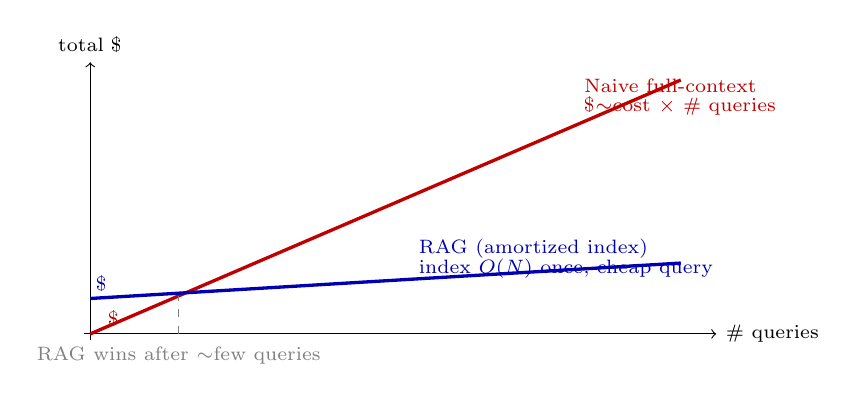
\begin{tikzpicture}[font=\small, scale=0.75]
  % axes
  \draw[->] (-0.1,0) -- (10.6,0) node[right, font=\scriptsize] {\# queries};
  \draw[->] (0,-0.1) -- (0,4.6) node[above, font=\scriptsize] {total \$};

  % Naive full-context curve: linear, steep
  \draw[red!75!black, very thick] (0,0.0) -- (10,4.3);
  \node[red!75!black, font=\scriptsize, anchor=west] at (8.2,4.2) {Naive full-context};
  \node[red!75!black, font=\scriptsize, anchor=west] at (8.2,3.85) {\$$\sim$cost $\times$ \# queries};

  % RAG curve: small upfront index cost, very flat query slope
  \draw[blue!70!black, very thick] (0,0.6) -- (10,1.2);
  \node[blue!70!black, font=\scriptsize, anchor=west] at (5.4,1.45) {RAG (amortized index)};
  \node[blue!70!black, font=\scriptsize, anchor=west] at (5.4,1.1) {index $O(N)$ once, cheap query};

  % markers on RAG curve at small \# queries
  \node[blue!70!black, font=\scriptsize] at (0.2,0.85) {\$};
  \node[red!75!black, font=\scriptsize] at (0.4,0.25) {\$};

  % crossover annotation
  \draw[gray, dashed] (1.5,0) -- (1.5,0.65);
  \node[gray, font=\scriptsize, anchor=north] at (1.5,-0.05) {RAG wins after $\sim$few queries};
\end{tikzpicture}
\end{center}

\smallskip
\begin{itemize}
\item \textbf{Naive full-context prompting:} cost scales \emph{linearly} with context size \emph{and} \# queries --- every question repays the full corpus token bill (Act 8.1's meter wall).
\item \textbf{RAG:} pay $O(N)$ embedding calls \emph{once} at index time; each query ships only the top-$K$ chunks ($\sim$1--5\% of the corpus). Marginal cost per query collapses.
\item \textbf{Per-token rates and the reproducibility tax:} Lec.\ 7 T4, ``Tokens, Cost, and Reproducibility.'' Past a handful of queries, index-once dominates on total spend \emph{and} latency.
\end{itemize}
\end{frame}

\begin{frame}{Bridge: The Pipeline Is Complete --- Now Make It Earn Its Keep}
\textbf{Act 4 closed the loop: retrieved chunks become cited evidence, the generator is contractually forced to ground, cite, and refuse --- and the decision matrix says when to fine-tune instead.}

\medskip
\begin{itemize}
\item \textbf{What changed:} the output is now \emph{auditable}. That is what makes RAG a research tool rather than a chat trick.

\medskip
\item \textbf{Rule to remember:} style, format, jargon $\to$ fine-tune; facts $\to$ retrieve.

\medskip
\item \textbf{Next --- Act 8.5 (APPLY):} the payoff. Six research corpora end to end, a classroom OLG demo you can run offline today, the six failure modes and their mitigations, RAGAS + human validation --- and the bridge to Lecture 9's agents.
\end{itemize}

\bigskip
\centering
\footnotesize\textit{Arc: Act 1 WALL $\to$ Act 2 INDEX $\to$ Act 3 RETRIEVE $\to$ \textbf{Act 4 GENERATE} $\to$ Act 5 APPLY.}
\end{frame}

\end{document}
